% =============================================================================
% TUTORIAL DE LA PLATAFORMA - IA Y APRENDIZAJE
% Guía para profesores y estudiantes
% Universidad de Extremadura - Curso 2025-2026
% =============================================================================

\documentclass[11pt,a4paper]{article}

% -----------------------------------------------------------------------------
% PAQUETES
% -----------------------------------------------------------------------------
\usepackage[utf8]{inputenc}
\usepackage[T1]{fontenc}
\usepackage[spanish]{babel}
\usepackage{mathpazo}
\usepackage{geometry}
\geometry{left=2.5cm, right=2.5cm, top=2.5cm, bottom=2.5cm}
\usepackage{setspace}
\setstretch{1.15}
\usepackage{xcolor}
\usepackage{tikz}
\usetikzlibrary{shapes, arrows.meta, positioning, babel}
\usepackage{booktabs}
\usepackage{tabularx}
\usepackage{enumitem}
\usepackage{graphicx}
\graphicspath{{screenshots/}}
\usepackage{hyperref}
\usepackage{fancyhdr}
\usepackage{tcolorbox}
\tcbuselibrary{skins, breakable}
\usepackage{fontawesome5}

% -----------------------------------------------------------------------------
% COLORES
% -----------------------------------------------------------------------------
\definecolor{azulUEx}{HTML}{1A365D}
\definecolor{verdeUEx}{HTML}{38A169}
\definecolor{grisClaro}{HTML}{F7FAFC}
\definecolor{azulClaro}{HTML}{EBF8FF}
\definecolor{verdeClaro}{HTML}{F0FFF4}
\definecolor{amarilloClaro}{HTML}{FFFFF0}
\definecolor{rojoClaro}{HTML}{FFF5F5}

% -----------------------------------------------------------------------------
% ENCABEZADOS
% -----------------------------------------------------------------------------
\pagestyle{fancy}
\fancyhf{}
\fancyhead[L]{\small\textsf{Tutorial de la Plataforma}}
\fancyhead[R]{\small\textsf{IA y Aprendizaje --- UEx}}
\fancyfoot[C]{\thepage}
\renewcommand{\headrulewidth}{0.4pt}

% -----------------------------------------------------------------------------
% COMANDOS Y ENTORNOS
% -----------------------------------------------------------------------------
\newcommand{\seccion}[1]{\section{\textsf{\textcolor{azulUEx}{#1}}}}
\newcommand{\subseccion}[1]{\subsection{\textsf{\textcolor{verdeUEx}{#1}}}}
\newcommand{\subsubseccion}[1]{\subsubsection{\textsf{#1}}}

% Paso numerado
\newcounter{paso}
\newcommand{\paso}[1]{%
    \stepcounter{paso}%
    \par\noindent\tikz[baseline=(num.base)]{
        \node[fill=azulUEx, text=white, circle, inner sep=0pt, minimum size=20pt, font=\bfseries\small] (num) {\thepaso};
    }\;\textbf{#1}\par\smallskip
}
\newcommand{\pasoVerde}[1]{%
    \stepcounter{paso}%
    \par\noindent\tikz[baseline=(num.base)]{
        \node[fill=verdeUEx, text=white, circle, inner sep=0pt, minimum size=20pt, font=\bfseries\small] (num) {\thepaso};
    }\;\textbf{#1}\par\smallskip
}
\newcommand{\resetpasos}{\setcounter{paso}{0}}

% Caja de consejo/nota
\newtcolorbox{nota}[1][Nota]{
    colback=amarilloClaro, colframe=yellow!60!black,
    fonttitle=\bfseries, title={#1},
    boxrule=0.5pt, arc=4pt, left=8pt, right=8pt,
    breakable
}

% Caja de información
\newtcolorbox{info}[1][]{
    colback=azulClaro, colframe=azulUEx!50,
    boxrule=0.5pt, arc=4pt, left=8pt, right=8pt,
    breakable, #1
}

% Caja de advertencia
\newtcolorbox{advertencia}[1][Importante]{
    colback=rojoClaro, colframe=red!40,
    fonttitle=\bfseries, title={#1},
    boxrule=0.5pt, arc=4pt, left=8pt, right=8pt,
    breakable
}

% Código inline
\newcommand{\codigo}[1]{\texttt{\textbf{#1}}}

% =============================================================================
% DOCUMENTO
% =============================================================================
\begin{document}

% -----------------------------------------------------------------------------
% PORTADA
% -----------------------------------------------------------------------------
\begin{titlepage}
    \centering
    \vspace*{2cm}

    {\Large\textsf{PROYECTO DE INNOVACIÓN DOCENTE}\par}
    \vspace{0.3cm}
    {\small Curso 2025--2026\par}

    \vspace{2cm}

    {\Huge\bfseries\textsf{\textcolor{azulUEx}{Tutorial de la Plataforma}}\par}

    \vspace{0.8cm}

    {\Large\textsf{Guía para Profesores y Estudiantes}\par}

    \vspace{1cm}

    {\large\textsf{IA y Aprendizaje}\par}

    \vspace{3cm}

    \begin{tikzpicture}
        \draw[azulUEx, line width=2pt] (-3,0) -- (3,0);
    \end{tikzpicture}

    \vspace{1cm}

    {\large Universidad de Extremadura\par}
    \vspace{0.3cm}
    {\normalsize Escuela Politécnica\par}

    \vspace{2cm}

    {\small Plataforma web: \url{https://gestor-investigacion-app.web.app}\par}

    \vfill
    {\footnotesize Última actualización: Abril 2026\par}
\end{titlepage}

% -----------------------------------------------------------------------------
% ÍNDICE
% -----------------------------------------------------------------------------
\tableofcontents
\newpage

% =============================================================================
% INTRODUCCIÓN
% =============================================================================
\seccion{Introducción}

Este documento es la guía de uso de la plataforma web del proyecto de innovación docente \textbf{<<IA y Aprendizaje>>}. La plataforma gestiona todo el flujo del estudio experimental: registro de participantes, inscripción en asignaturas, recogida de cuestionarios y evaluación con rúbricas.

\begin{info}
\textbf{URL de acceso:} \url{https://gestor-investigacion-app.web.app}
\end{info}

\subseccion{Roles en la plataforma}

La plataforma tiene tres roles:

\begin{itemize}[leftmargin=2cm]
    \item[\textbf{Administrador}] Gestiona centros universitarios, profesores y tiene acceso global a los datos de investigación.
    \item[\textbf{Profesor}] Crea asignaturas, gestiona estudiantes, evalúa con rúbricas y supervisa el progreso.
    \item[\textbf{Estudiante}] Se inscribe en asignaturas y completa los cuestionarios del estudio.
\end{itemize}

% =============================================================================
% REGISTRO Y ACCESO
% =============================================================================
\seccion{Registro y acceso}

\subseccion{Registro (primera vez)}

Para participar necesitas un \textbf{email institucional} de una universidad registrada en el proyecto (por ejemplo, \codigo{@unex.es} o \codigo{@alumnos.unex.es}).

\resetpasos
\paso{Accede a la página de login}
Ve a \url{https://gestor-investigacion-app.web.app/app/login.html} y haz clic en \textbf{<<¿No tienes cuenta? Regístrate>>}.

\paso{Rellena el formulario}
Introduce tu email institucional y elige una contraseña (mínimo 6 caracteres). Confírmala escribiéndola de nuevo.

\paso{Verifica tu email}
Recibirás un email de verificación. Haz clic en el enlace para activar tu cuenta.

\pasoVerde{Listo}
Ya puedes iniciar sesión con tu email y contraseña.

\begin{figure}[ht]
    \centering
    \fbox{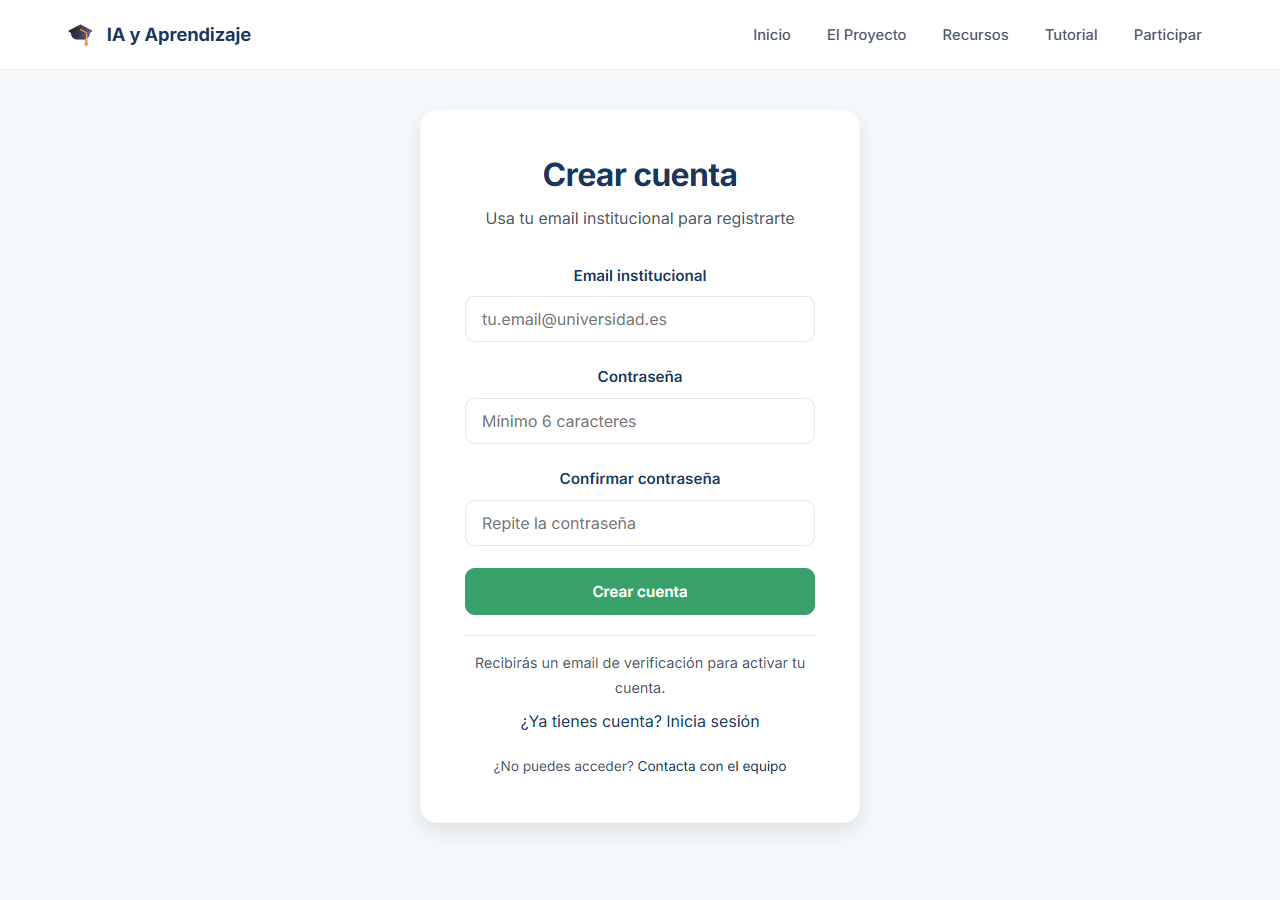
\includegraphics[width=0.65\textwidth]{03_registro.png}}
    \caption{Formulario de registro con email institucional y contraseña.}
\end{figure}

\begin{nota}[Nota para profesores]
Si te registras directamente, tu cuenta se creará como \textit{estudiante}. El administrador del proyecto debe asignarte el rol de \textit{profesor} desde el panel de administración. Contacta con el coordinador del proyecto para que te dé de alta como profesor.
\end{nota}

\begin{nota}[Email en spam]
Si no recibes el email de verificación, revisa la carpeta de \textbf{spam} o \textbf{correo no deseado}. El email proviene de Firebase (noreply@gestor-investigacion-app.firebaseapp.com).
\end{nota}

\subseccion{Iniciar sesión}

Hay dos formas de acceder:

\begin{figure}[ht]
    \centering
    \fbox{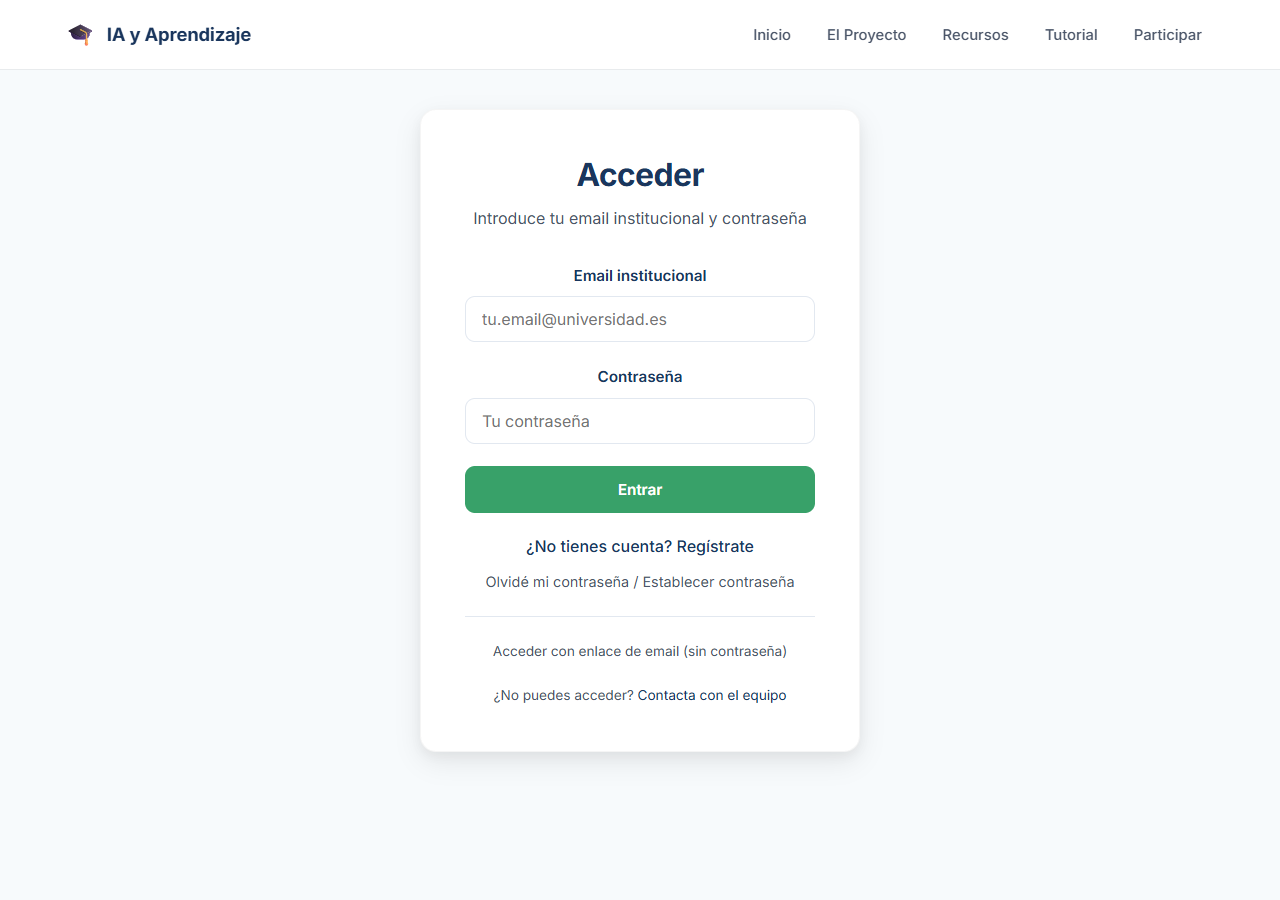
\includegraphics[width=0.65\textwidth]{02_login.png}}
    \caption{Página de inicio de sesión con las opciones de acceso.}
\end{figure}

\subsubseccion{Con contraseña (recomendado)}
\resetpasos
\paso{Introduce tu email y contraseña en la página de login y pulsa <<Entrar>>.}
El sistema te redirigirá automáticamente a tu panel según tu rol.

\subsubseccion{Con enlace de email (magic link)}
\resetpasos
\paso{Haz clic en <<Acceder con enlace de email (sin contraseña)>>.}

\paso{Introduce tu email institucional.}

\paso{Recibirás un enlace de acceso directo en tu email. Haz clic para entrar.}

\begin{info}
El acceso con enlace de email es útil si no recuerdas tu contraseña o prefieres no usar una. Sin embargo, depende de que el email llegue correctamente a tu bandeja.
\end{info}

\subseccion{Gestión de contraseña}

\subsubseccion{Olvidé mi contraseña}
\resetpasos
\paso{En la página de login, haz clic en <<Olvidé mi contraseña / Establecer contraseña>>.}
\paso{Introduce tu email y pulsa <<Enviar enlace>>.}
\paso{Recibirás un email con un enlace para crear una nueva contraseña.}

\subsubseccion{Usuarios existentes (sin contraseña)}
Si accedías previamente solo con magic link y quieres establecer una contraseña, usa el mismo proceso de <<Establecer contraseña>>. Tu cuenta se actualizará y podrás elegir entre ambos métodos de acceso.

% =============================================================================
% GUÍA PARA PROFESORES
% =============================================================================
\seccion{Guía para profesores}

\subseccion{Panel de profesor}

Al iniciar sesión como profesor, accedes a tu panel donde puedes:
\begin{itemize}
    \item Crear y gestionar asignaturas
    \item Añadir estudiantes o compartir códigos de invitación
    \item Ver el progreso de los cuestionarios
    \item Evaluar trabajos con rúbricas
\end{itemize}

\begin{figure}[ht]
    \centering
    \fbox{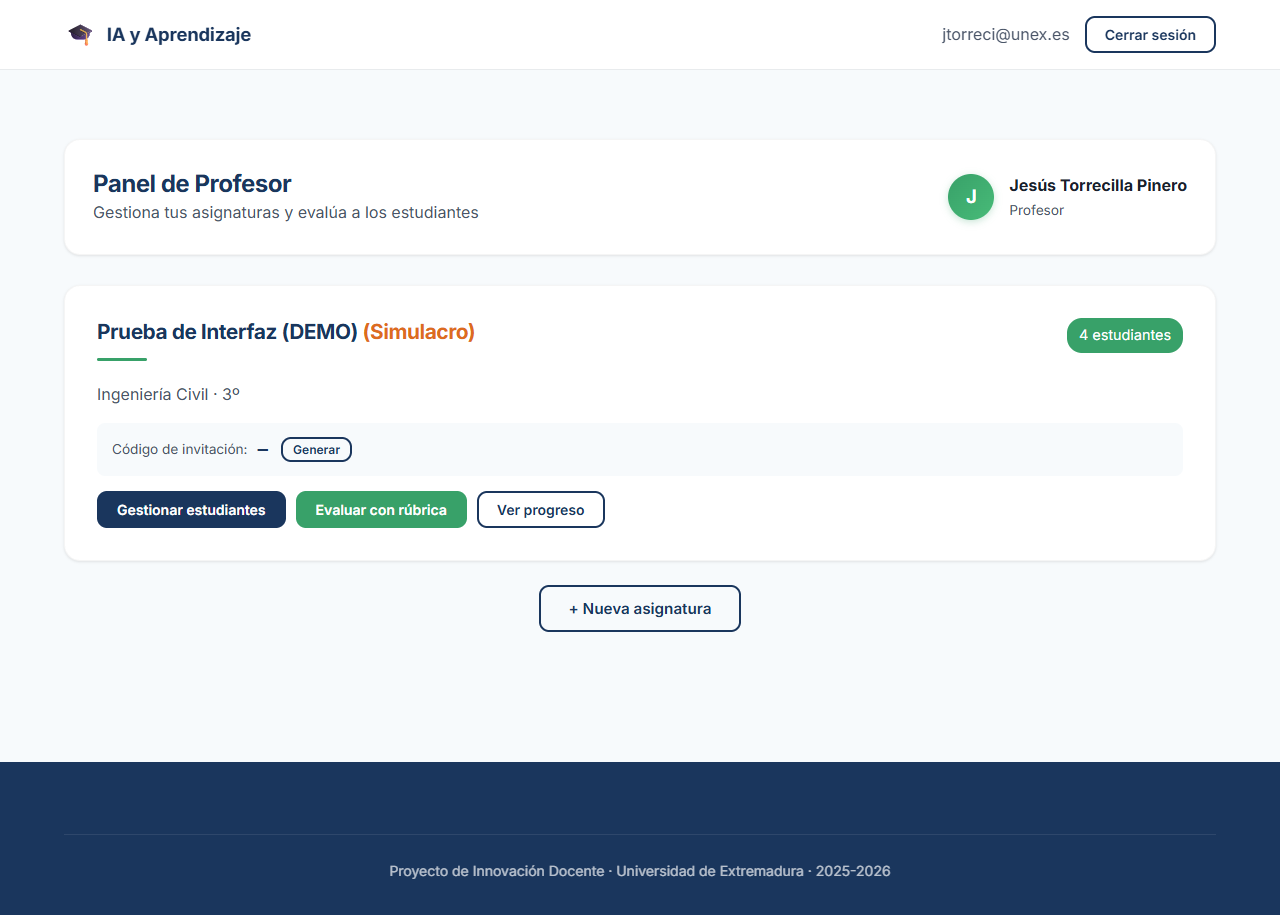
\includegraphics[width=0.85\textwidth]{10_profesor_panel.png}}
    \caption{Panel de profesor con tarjeta de asignatura, código de invitación y botones de acción.}
\end{figure}

\subseccion{Crear una asignatura}
\resetpasos
\paso{En tu panel, pulsa <<+ Nueva asignatura>> o <<Crear asignatura>>.}
\paso{Rellena el nombre de la asignatura, la titulación y el curso.}
\paso{Si es una asignatura de prueba, marca la casilla <<Simulacro>>.}
\pasoVerde{Al crear la asignatura se generará automáticamente un \textbf{código de invitación} de 6 caracteres.}

\begin{info}
El código de invitación aparece en la tarjeta de cada asignatura. Puedes copiarlo con el botón <<Copiar>> y compartirlo con tus estudiantes por el medio que prefieras (en clase, campus virtual, email...).
\end{info}

\begin{figure}[ht]
    \centering
    \fbox{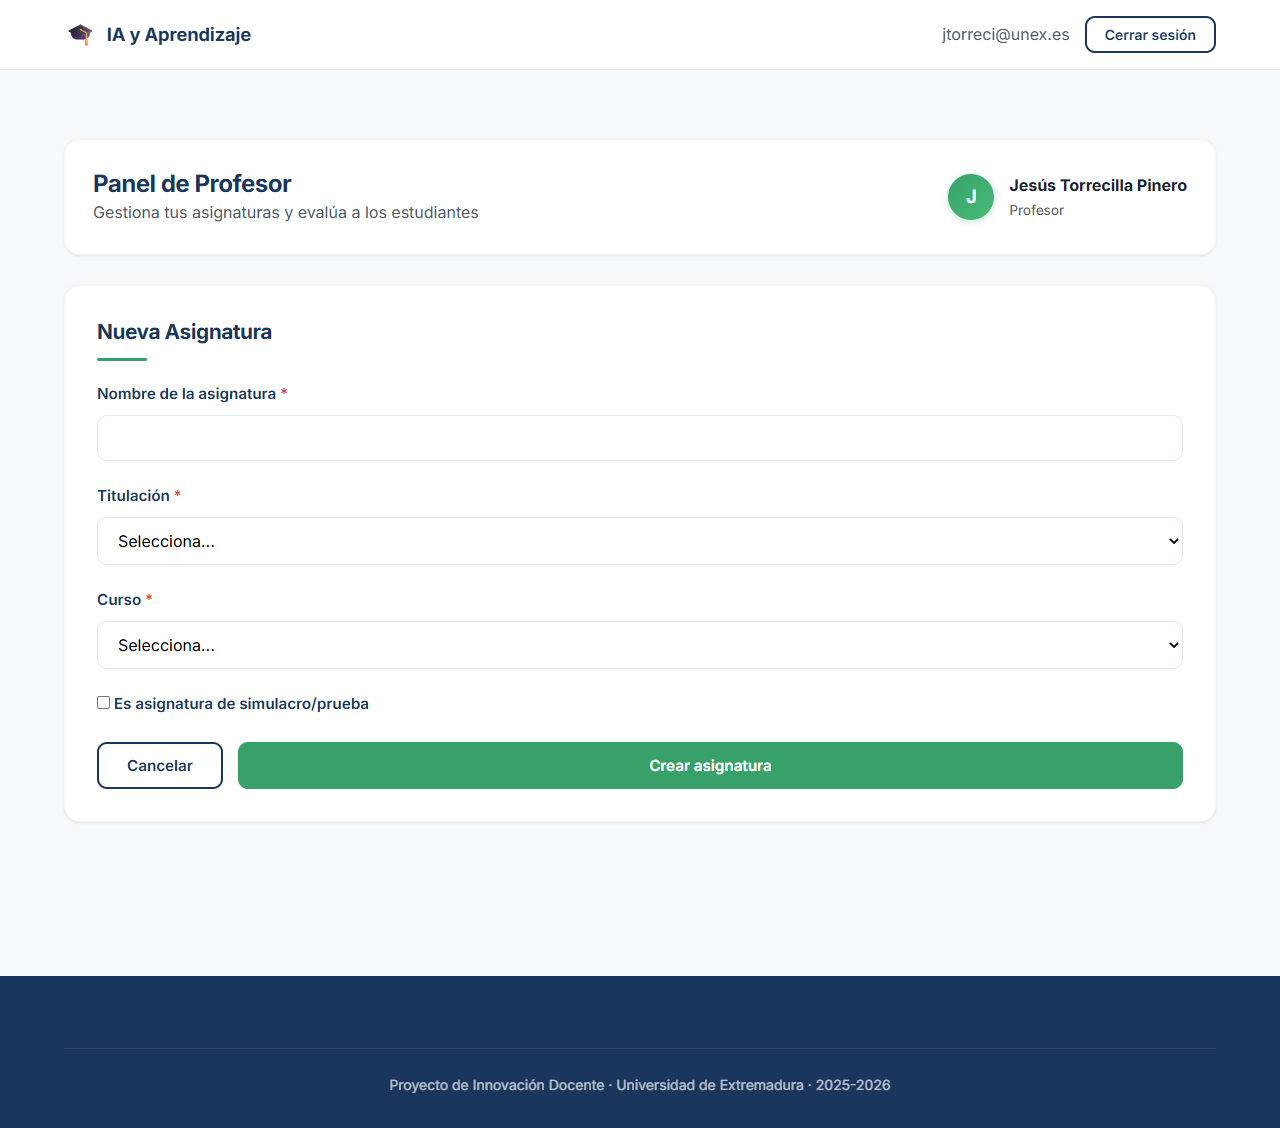
\includegraphics[width=0.85\textwidth]{20_prof_crear_asignatura.png}}
    \caption{Formulario de creación de asignatura con nombre, titulación, curso y opción de simulacro.}
\end{figure}

\subseccion{Gestionar estudiantes}

Hay dos formas de inscribir estudiantes en una asignatura:

\subsubseccion{Opción A: Código de invitación (recomendado)}

Comparte el código de invitación con tus estudiantes. Ellos se registran en la plataforma y usan el código para inscribirse por sí mismos desde su panel de estudiante.

\textbf{Ventaja:} No necesitas recoger ni escribir los emails de los estudiantes.

\subsubseccion{Opción B: Alta manual por el profesor}
\resetpasos
\paso{En la tarjeta de tu asignatura, pulsa <<Gestionar estudiantes>>.}
\paso{En el campo de texto, escribe los emails institucionales de los estudiantes (uno por línea).}
\paso{Pulsa <<Añadir estudiantes>>.}

\begin{nota}[Protección de roles]
El sistema comprueba automáticamente si un email corresponde a un profesor o administrador. Si es así, \textbf{no se modifica su rol} y verás un mensaje informativo. Igualmente, si el estudiante ya estaba registrado, se inscribirá en la asignatura sin duplicar su cuenta.
\end{nota}

\begin{nota}[Sin grupo inicial]
Los estudiantes se inscriben \textbf{sin grupo asignado}. Debes asignarles grupo manualmente (ver siguiente sección).
\end{nota}

\subseccion{Asignar grupos A/B}

La asignación de grupos es \textbf{manual}, lo que te da control total sobre la composición de cada grupo.

\resetpasos
\paso{En la tarjeta de tu asignatura, pulsa <<Gestionar estudiantes>>.}
\paso{Verás una tabla con todos los estudiantes inscritos. Cada fila tiene dos botones de radio: \textbf{Grupo A} y \textbf{Grupo B}.}
\paso{Marca el grupo de cada estudiante. Si no marcas ninguno, ese estudiante \textbf{no participará} en el experimento (queda inscrito pero sin acceso a los cuestionarios).}
\pasoVerde{Pulsa <<Guardar asignación de grupos>>.}

\begin{center}
\begin{tabular}{lcc}
    \toprule
    & \textbf{Reto 1} & \textbf{Reto 2} \\
    \midrule
    \textbf{Grupo A} & Sin IA & Con IA \\
    \textbf{Grupo B} & Con IA & Sin IA \\
    \bottomrule
\end{tabular}
\end{center}

Este diseño cruzado permite que cada estudiante sea su propio control, comparando su rendimiento con y sin IA.

\begin{advertencia}[Bloqueo de grupo]
Una vez que un estudiante haya completado algún cuestionario, su grupo quedará \textbf{bloqueado} (aparece un candado en la interfaz) para garantizar la integridad del diseño cruzado. El grupo no podrá modificarse a partir de ese momento.
\end{advertencia}

\begin{figure}[ht]
    \centering
    \fbox{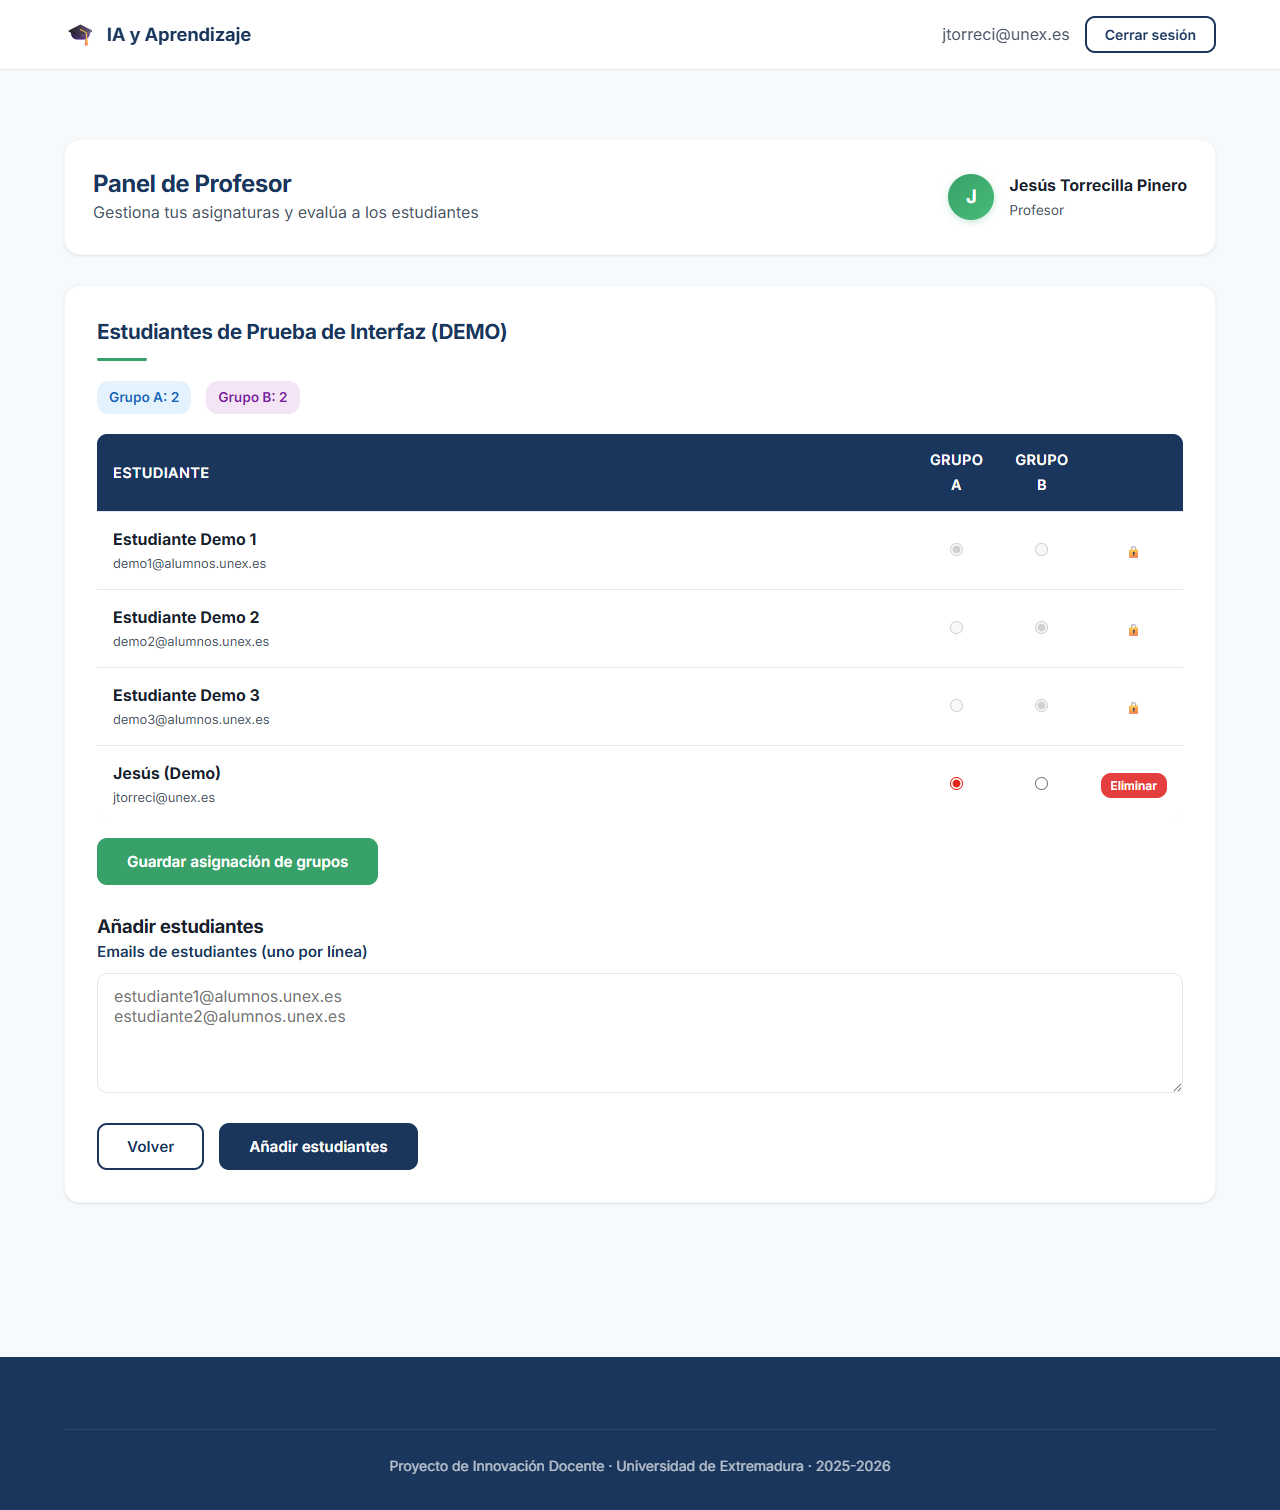
\includegraphics[width=0.85\textwidth]{21_prof_gestionar_estudiantes.png}}
    \caption{Gestión de estudiantes con asignación manual de grupos A/B. Los candados indican grupos bloqueados por cuestionarios completados.}
\end{figure}

\subseccion{Códigos de invitación}

Cada asignatura tiene un código único de 6 caracteres (por ejemplo, \codigo{A3X7K9}).

\begin{itemize}
    \item El código aparece en la tarjeta de la asignatura en tu panel.
    \item Usa el botón <<Copiar>> para copiarlo al portapapeles.
    \item Si una asignatura no tiene código (creada antes de esta funcionalidad), pulsa <<Generar>>.
    \item Se excluyen caracteres ambiguos (0/O, 1/I/L) para facilitar la lectura.
\end{itemize}

\subseccion{Ver progreso}
\resetpasos
\paso{En la tarjeta de tu asignatura, pulsa <<Ver progreso>>.}
\paso{Verás un resumen con barras de progreso para cada cuestionario y una tabla detallada por estudiante con indicadores de completado.}

\begin{figure}[ht]
    \centering
    \fbox{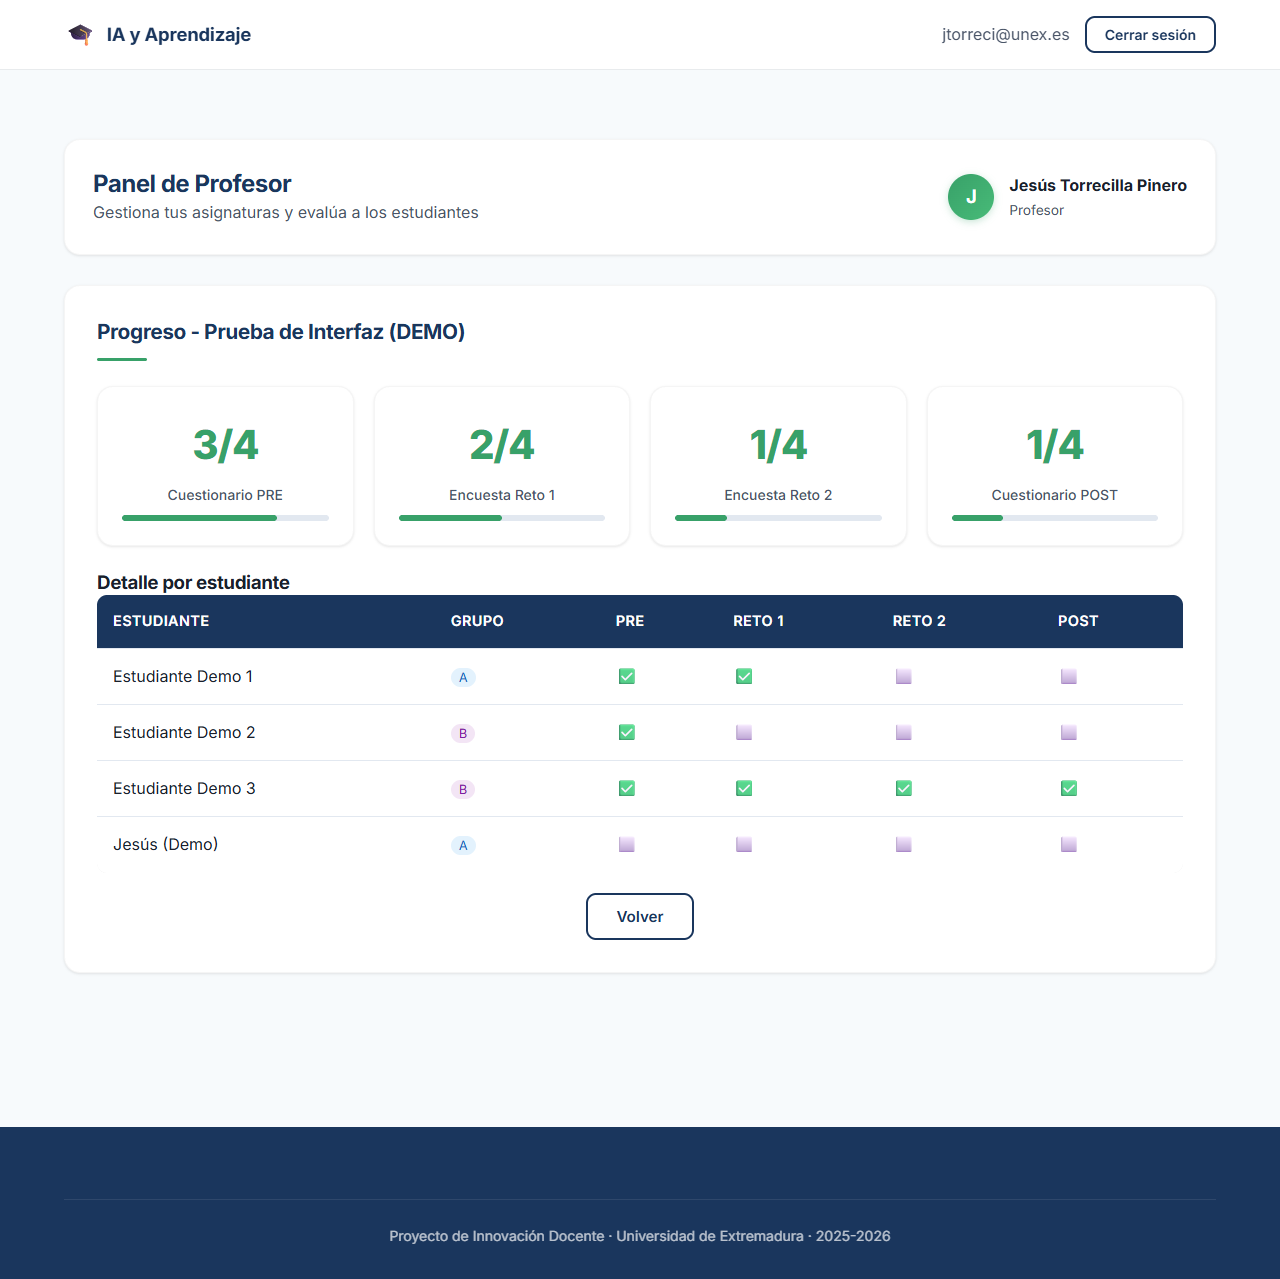
\includegraphics[width=0.85\textwidth]{23_prof_ver_progreso.png}}
    \caption{Vista de progreso con barras de completado por cuestionario y detalle por estudiante.}
\end{figure}

\subseccion{Evaluar con rúbrica}
\resetpasos
\paso{Pulsa <<Evaluar con rúbrica>> en la tarjeta de la asignatura.}
\paso{Selecciona el estudiante, el reto a evaluar (1 o 2) y la condición (con/sin IA).}
\paso{Puntúa cada criterio del 1 al 4:}

\begin{center}
\begin{tabularx}{\textwidth}{Xcccc}
    \toprule
    \textbf{Criterio} & \textbf{1} & \textbf{2} & \textbf{3} & \textbf{4} \\
    \midrule
    Comprensión del problema & Insuf. & Suf. & Bueno & Excelente \\
    Calidad de la solución & Insuf. & Suf. & Bueno & Excelente \\
    Razonamiento & Insuf. & Suf. & Bueno & Excelente \\
    Uso de conceptos & Insuf. & Suf. & Bueno & Excelente \\
    Presentación & Insuf. & Suf. & Bueno & Excelente \\
    Originalidad & Insuf. & Suf. & Bueno & Excelente \\
    \bottomrule
\end{tabularx}
\end{center}

\paso{Añade observaciones opcionales y pulsa <<Guardar evaluación>>.}

\begin{figure}[ht]
    \centering
    \fbox{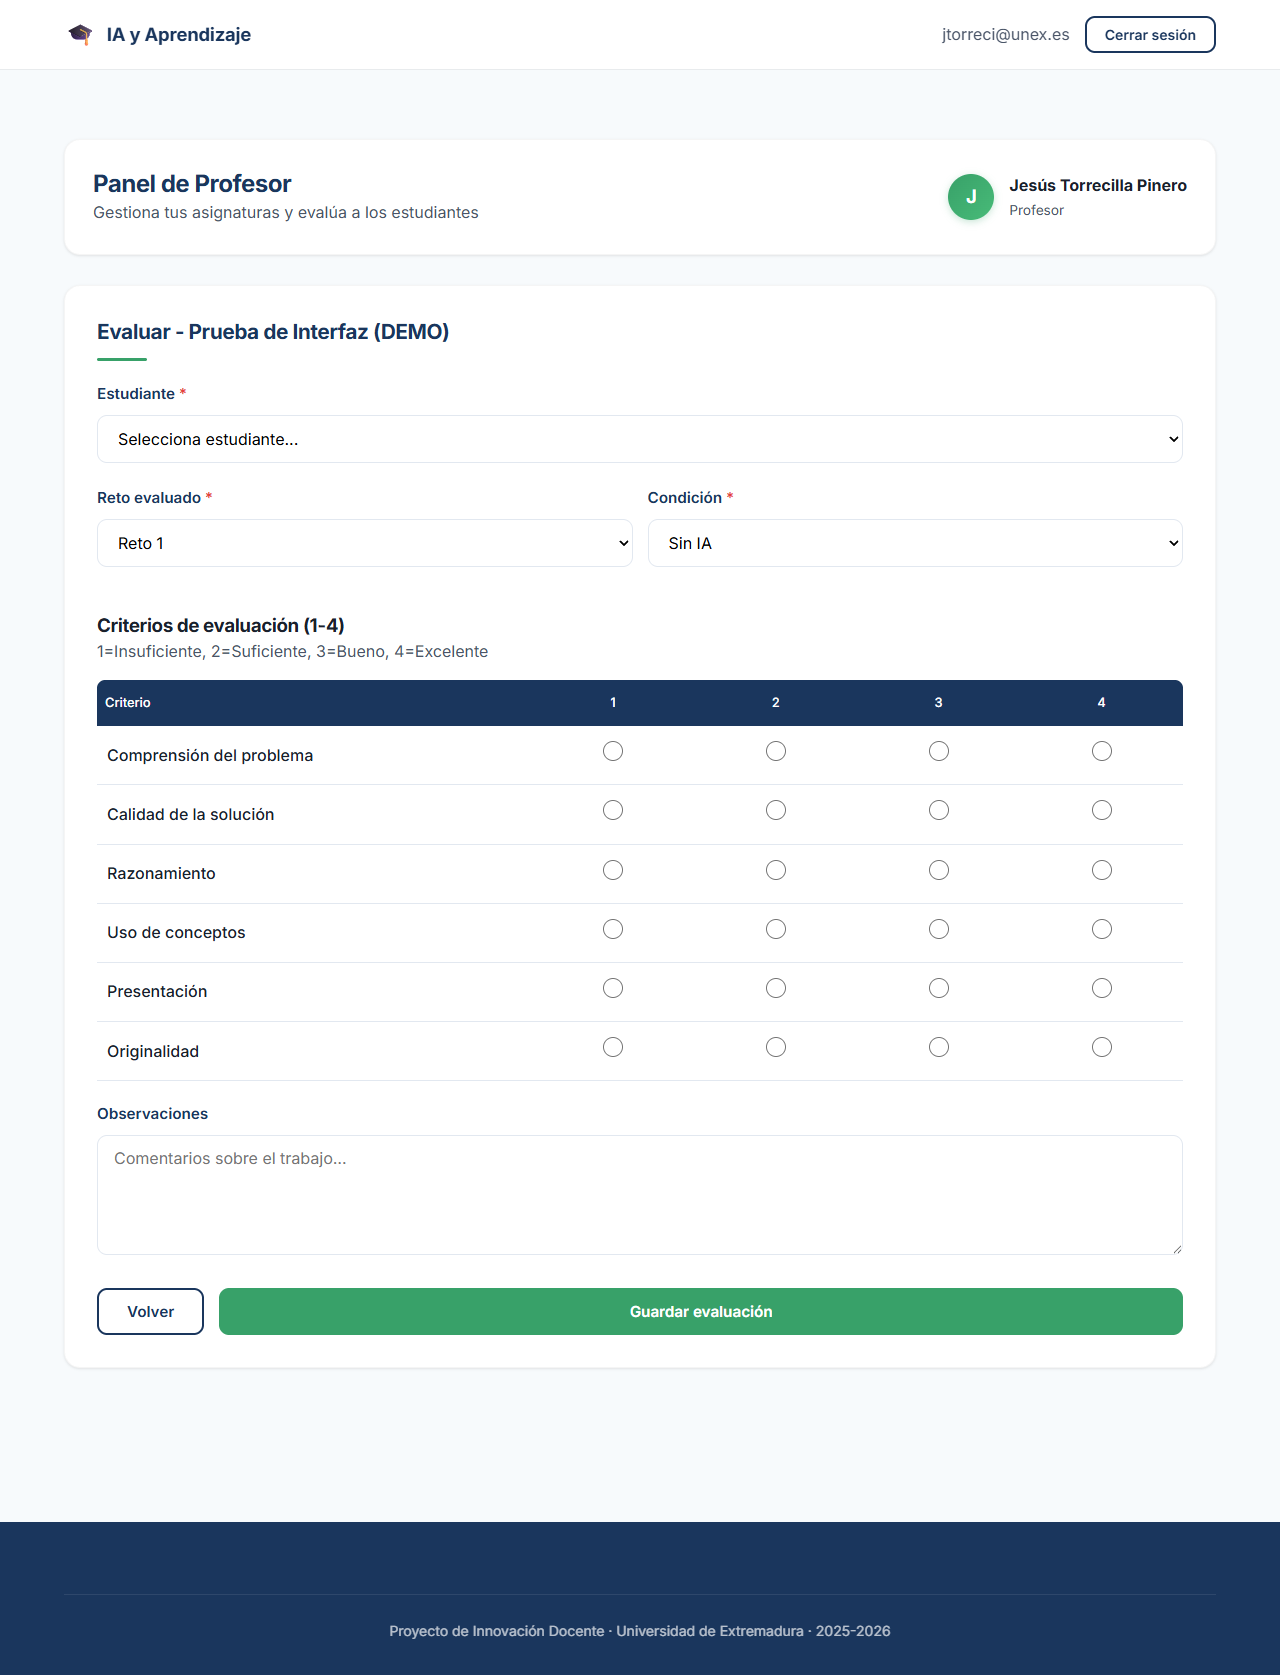
\includegraphics[width=0.85\textwidth]{22_prof_evaluar_rubrica.png}}
    \caption{Formulario de evaluación con rúbrica: selección de estudiante, reto, y puntuación por criterio (1--4).}
\end{figure}

\begin{info}
Las evaluaciones se vinculan al estudiante mediante un \textbf{código anónimo} (SHA-256). En el análisis de datos, las calificaciones no se asocian directamente a identidades personales.
\end{info}

% =============================================================================
% GUÍA PARA ESTUDIANTES
% =============================================================================
\seccion{Guía para estudiantes}

\subseccion{Panel de estudiante}

Al iniciar sesión como estudiante, accedes a tu panel donde puedes:
\begin{itemize}
    \item Inscribirte en asignaturas usando códigos de invitación
    \item Ver tus asignaturas, grupo asignado y progreso
    \item Completar los cuestionarios del estudio
\end{itemize}

\begin{figure}[ht]
    \centering
    \fbox{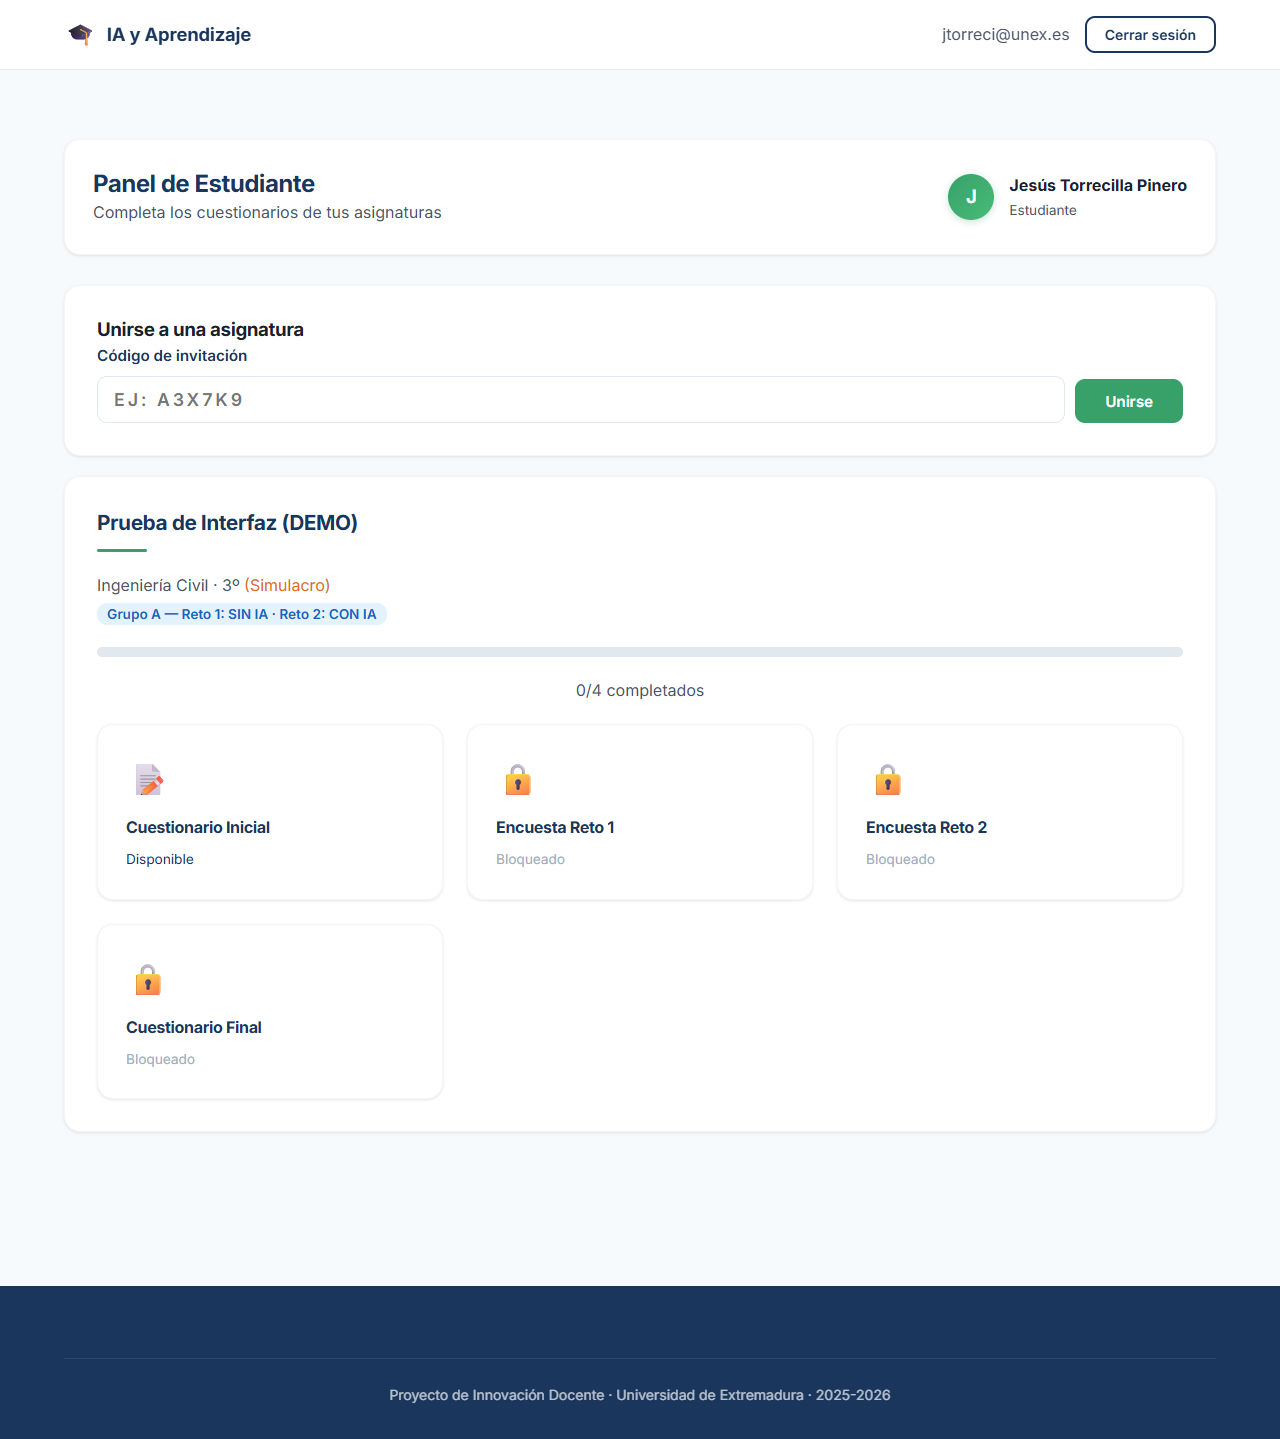
\includegraphics[width=0.85\textwidth]{11_estudiante_panel.png}}
    \caption{Panel de estudiante con campo de código de invitación y cuestionarios de una asignatura.}
\end{figure}

\subseccion{Inscribirse en una asignatura}
\resetpasos
\paso{Regístrate en la plataforma con tu email institucional (ver sección~\ref{sec:registro}).}
\paso{Inicia sesión y accede a tu panel de estudiante.}
\paso{En la parte superior verás el campo <<Código de invitación>>. Introduce el código de 6 caracteres que te ha dado tu profesor.}
\pasoVerde{Pulsa <<Unirse>>. Quedarás inscrito en la asignatura.}

\begin{nota}[Asignación de grupo]
Al inscribirte no se te asigna grupo automáticamente. Tu profesor te asignará al \textbf{Grupo A o B} desde su panel. Hasta entonces, verás un mensaje de <<Pendiente de asignación de grupo>> y no podrás acceder a los cuestionarios.
\end{nota}

Puedes inscribirte en varias asignaturas si participas en más de una.

\subseccion{Completar cuestionarios}

Cada asignatura tiene \textbf{4 cuestionarios} que se desbloquean en orden secuencial:

\resetpasos
\paso{Cuestionario Inicial (PRE)}
Preguntas sobre tu experiencia previa con IA, actitudes y expectativas. Incluye el consentimiento de participación en el estudio.

\begin{figure}[ht]
    \centering
    \fbox{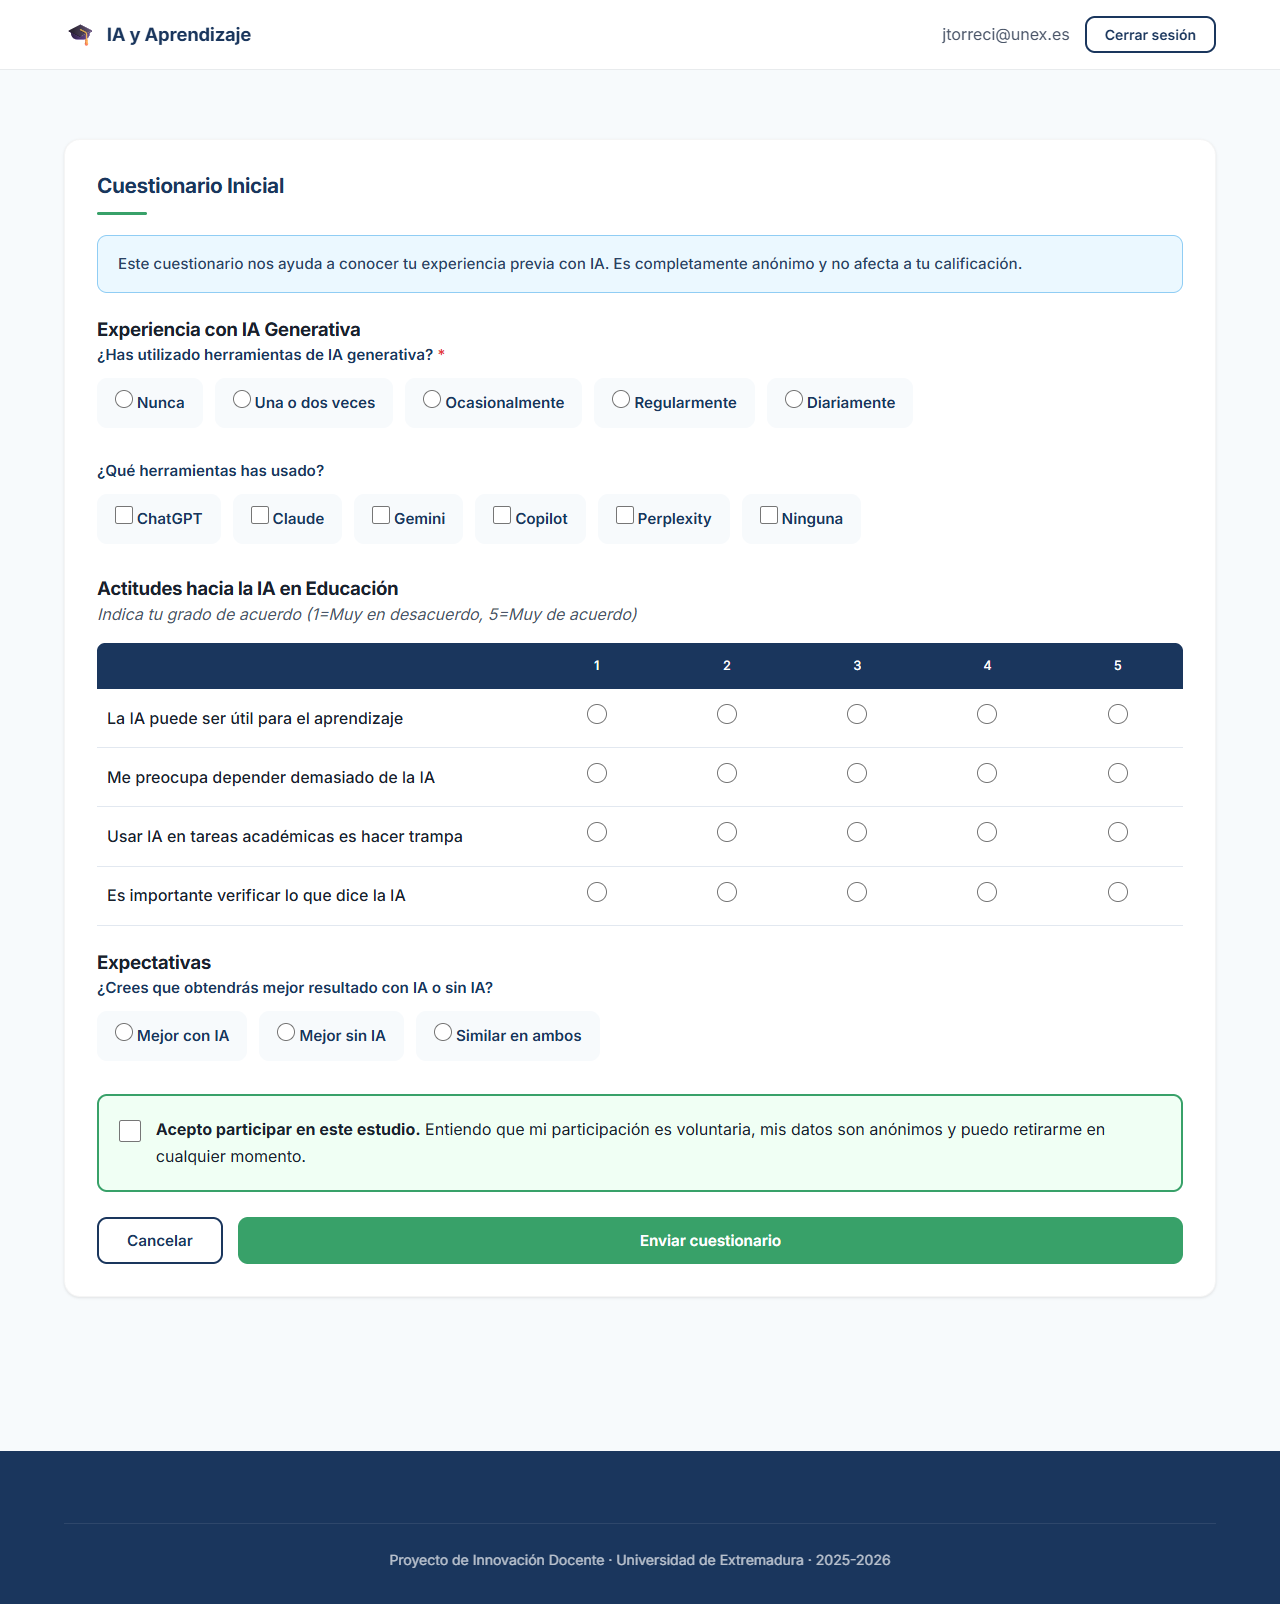
\includegraphics[width=0.85\textwidth]{30_est_cuestionario_pre.png}}
    \caption{Cuestionario Inicial (PRE): experiencia con IA, actitudes (escala Likert), expectativas y consentimiento.}
\end{figure}

\paso{Encuesta Reto 1}
Después de completar el primer reto de la asignatura, responde sobre dificultad, tiempo dedicado, satisfacción y aprendizaje. Tu grupo determina si usaste IA o no.

\begin{figure}[ht]
    \centering
    \fbox{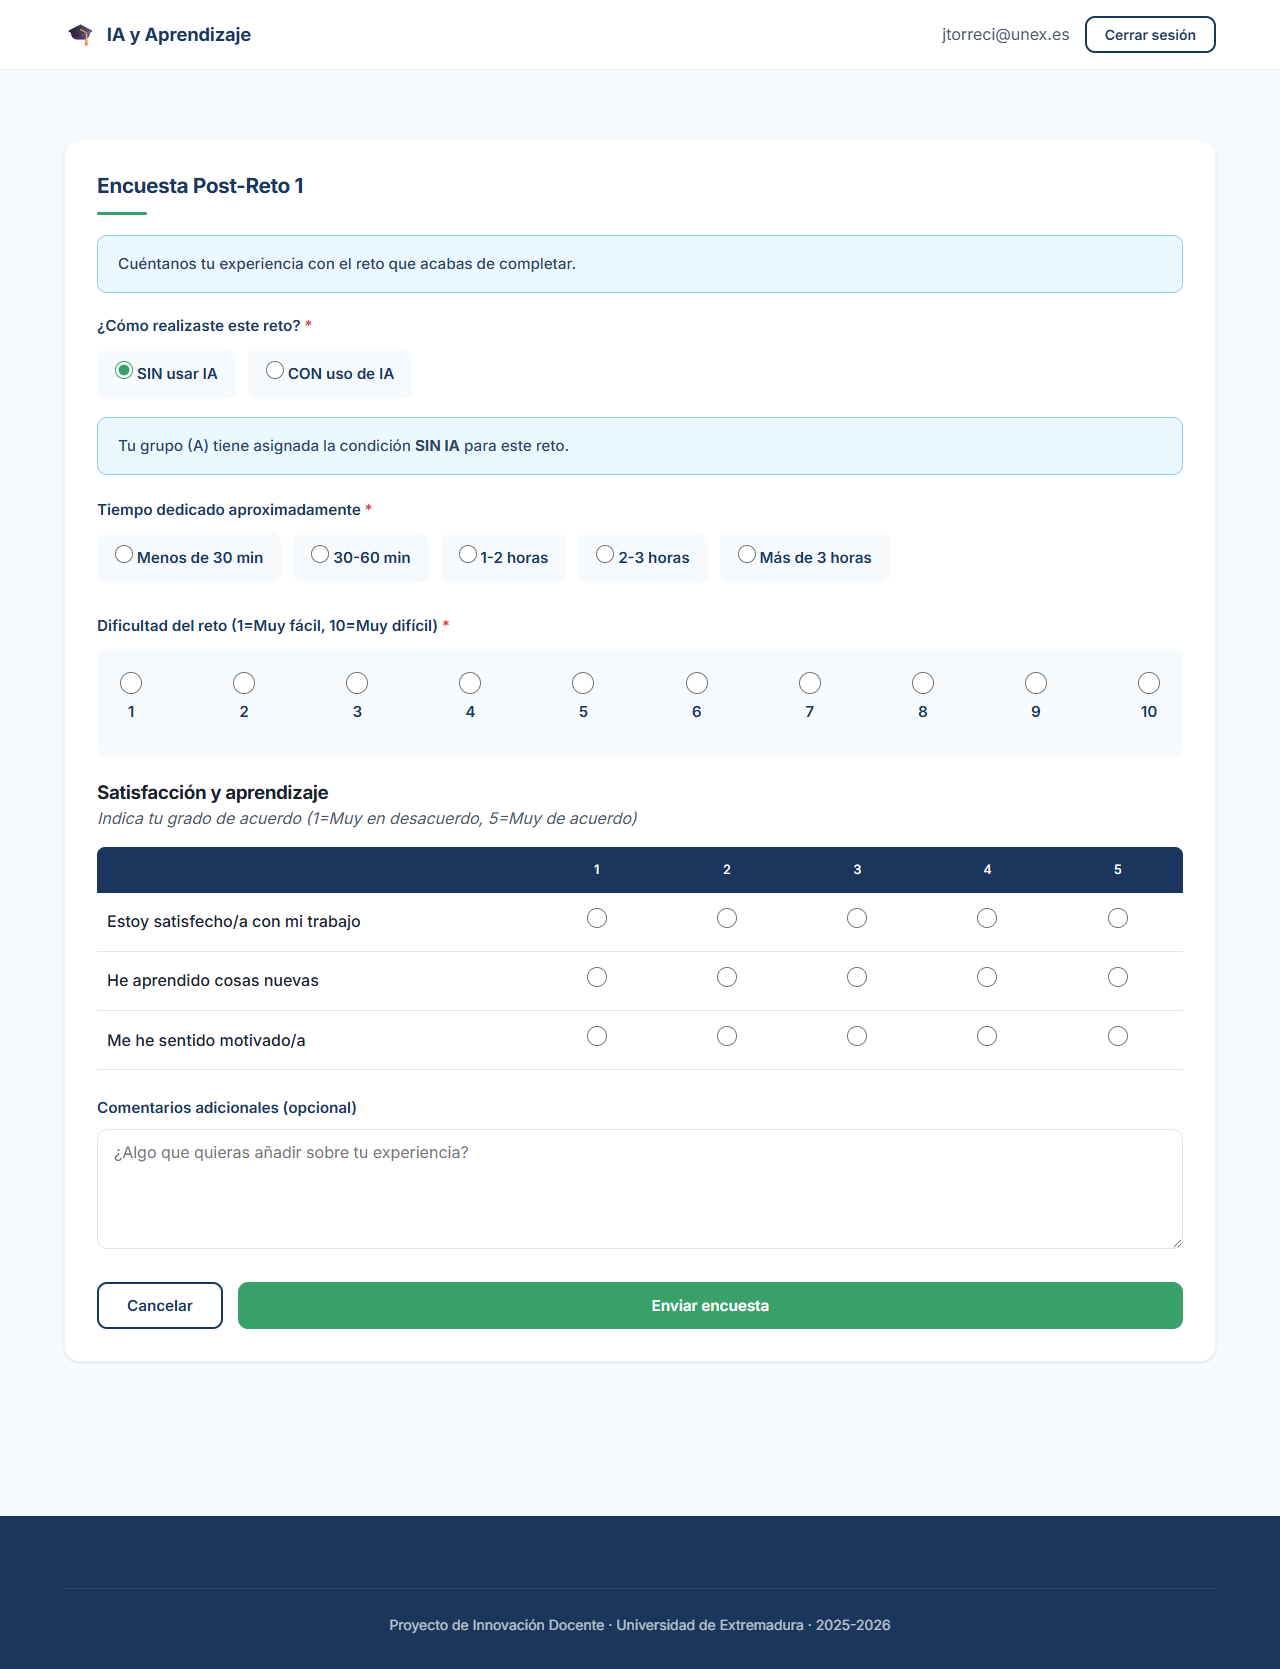
\includegraphics[width=0.85\textwidth]{31_est_encuesta_reto.png}}
    \caption{Encuesta post-reto: condición asignada, tiempo, dificultad, satisfacción y preguntas específicas sobre uso de IA.}
\end{figure}

\paso{Encuesta Reto 2}
Igual que la anterior, pero con la condición opuesta: si en el Reto~1 trabajaste con IA, en el Reto~2 lo harás sin IA, y viceversa.

\pasoVerde{Cuestionario Final (POST)}
Reflexión global comparando ambas experiencias y tus preferencias para el futuro.

\begin{figure}[ht]
    \centering
    \fbox{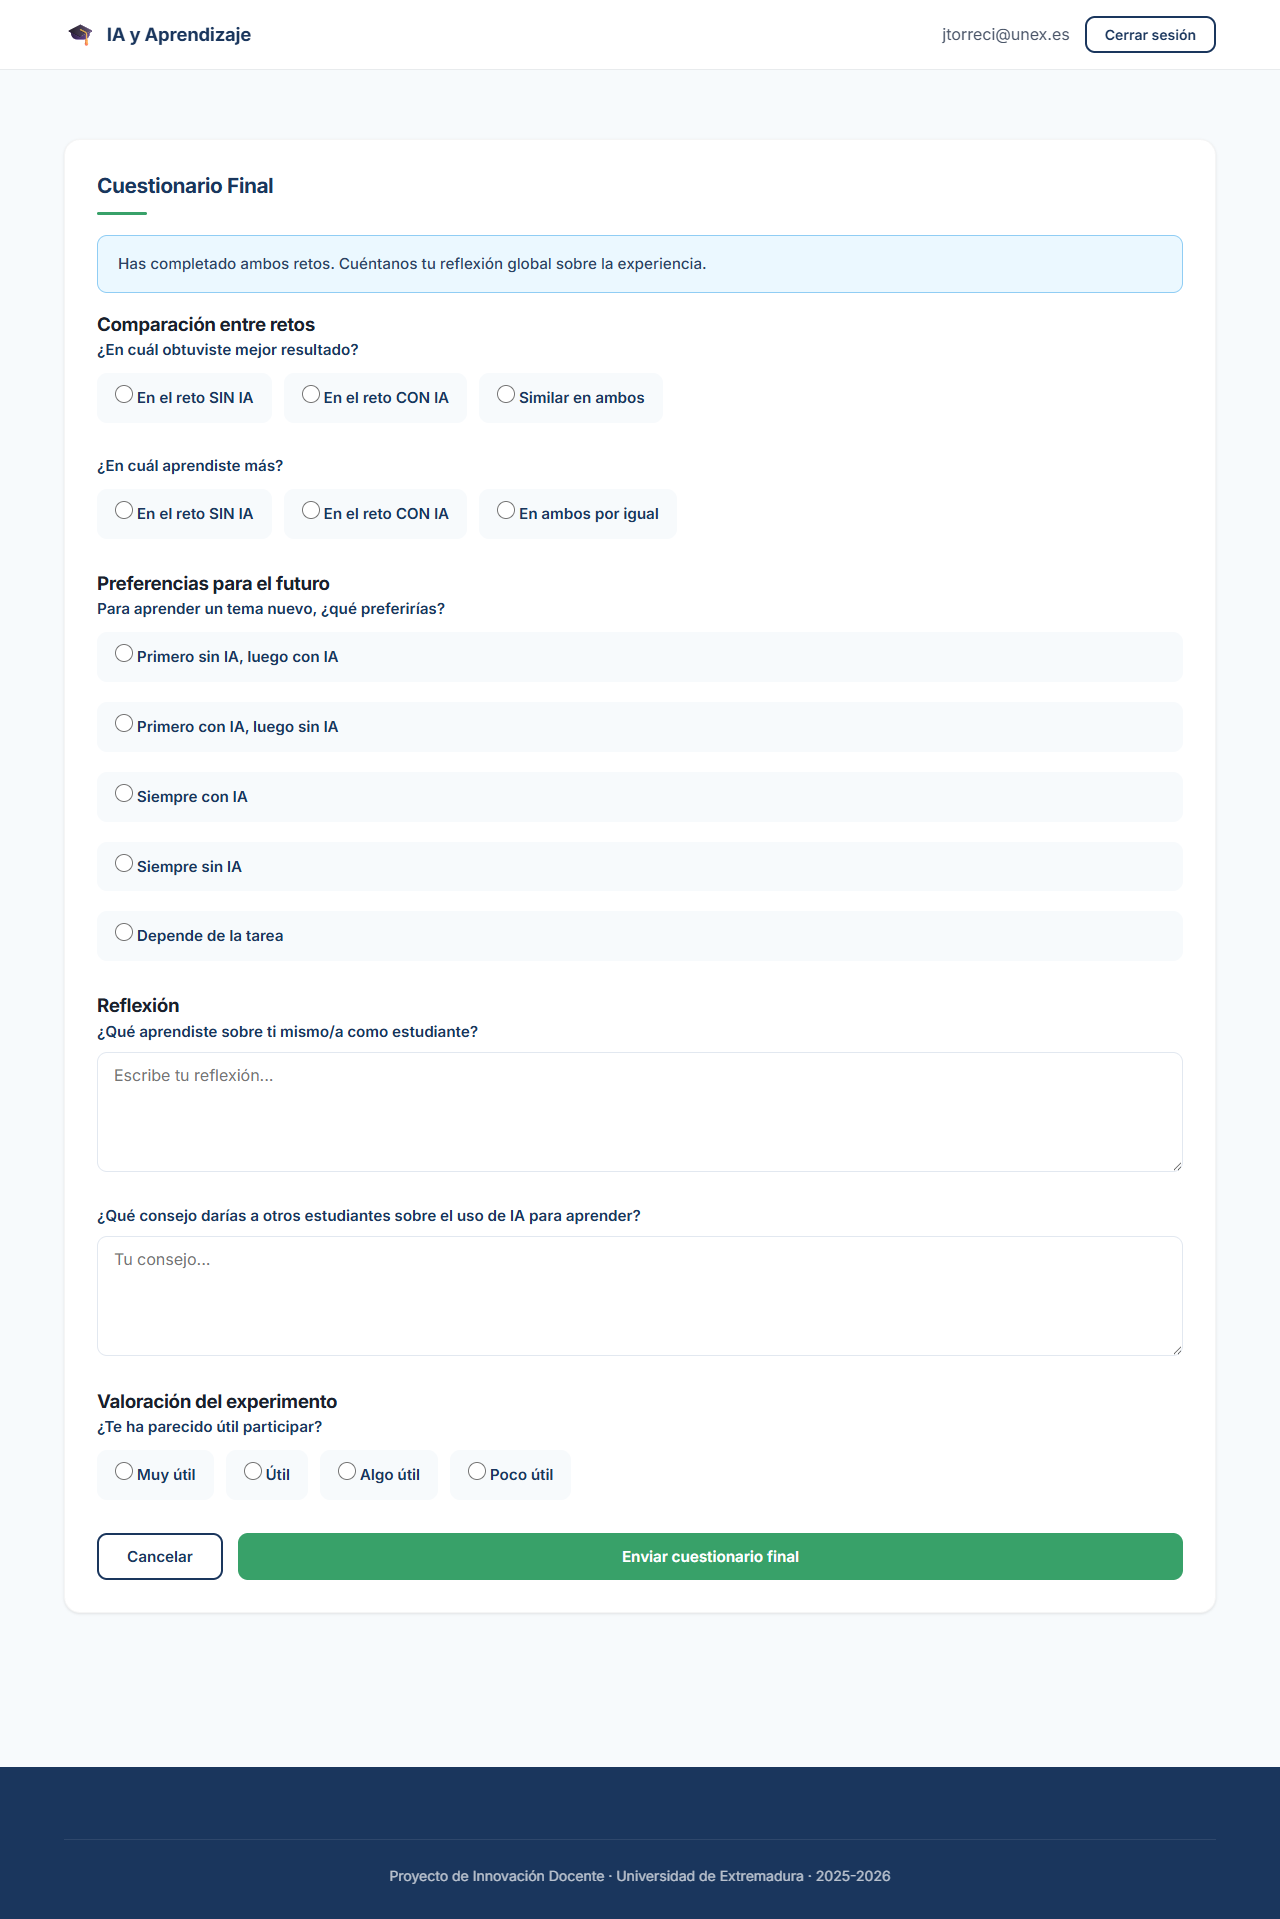
\includegraphics[width=0.85\textwidth]{32_est_cuestionario_post.png}}
    \caption{Cuestionario Final (POST): comparación entre retos, preferencias de aprendizaje y reflexión personal.}
\end{figure}

\begin{nota}[Anonimato]
Tus respuestas son \textbf{completamente anónimas}. Se asocian a un código generado automáticamente, no a tu nombre ni email. Tu profesor \textbf{no puede ver tus respuestas} individuales a los cuestionarios.
\end{nota}

\subseccion{Flujo completo del estudiante}

\begin{center}
\begin{tikzpicture}[
    node distance=0.8cm,
    box/.style={rectangle, draw=azulUEx, fill=azulClaro, rounded corners=4pt, text width=10cm, minimum height=1cm, align=center, font=\small},
    boxfinal/.style={rectangle, draw=verdeUEx, fill=verdeClaro, rounded corners=4pt, text width=10cm, minimum height=1cm, align=center, font=\small},
    flecha/.style={-{Stealth[length=6pt]}, thick, azulUEx!60}
]
    \node[box] (r1) {1. Te registras con tu email institucional y contraseña};
    \node[box, below=of r1] (r2) {2. Verificas tu email haciendo clic en el enlace};
    \node[box, below=of r2] (r3) {3. Inicias sesión y usas el código de invitación para inscribirte};
    \node[box, below=of r3] (r4) {4. Tu profesor te asigna a Grupo A o B};
    \node[box, below=of r4] (r5) {5. Completas el Cuestionario Inicial (PRE)};
    \node[box, below=of r5] (r6) {6. Realizas el Reto 1 y rellenas la encuesta};
    \node[box, below=of r6] (r7) {7. Realizas el Reto 2 (condición opuesta) y rellenas la encuesta};
    \node[boxfinal, below=of r7] (r8) {8. Completas el Cuestionario Final (POST)};

    \draw[flecha] (r1) -- (r2);
    \draw[flecha] (r2) -- (r3);
    \draw[flecha] (r3) -- (r4);
    \draw[flecha] (r4) -- (r5);
    \draw[flecha] (r5) -- (r6);
    \draw[flecha] (r6) -- (r7);
    \draw[flecha] (r7) -- (r8);
\end{tikzpicture}
\end{center}

% =============================================================================
% PREGUNTAS FRECUENTES
% =============================================================================
\seccion{Preguntas frecuentes}

\subseccion{Generales}

\textbf{¿Qué navegador debo usar?}\\
La plataforma funciona en cualquier navegador moderno (Chrome, Firefox, Edge, Safari). Se recomienda tener el navegador actualizado.

\textbf{¿Puedo acceder desde el móvil?}\\
Sí, la plataforma es responsive y se adapta a dispositivos móviles y tablets.

\textbf{¿Qué hago si el email de verificación no llega?}\\
Revisa la carpeta de spam. Si sigue sin aparecer, intenta iniciar sesión: el sistema te ofrecerá reenviar el email de verificación. También puedes usar la opción <<Acceder con enlace de email>> como alternativa.

\subseccion{Para profesores}

\textbf{¿Puedo añadir a otro profesor como estudiante?}\\
No. El sistema detecta automáticamente si un email pertenece a un profesor o administrador y lo protege. Verás un mensaje informativo indicando que se ha omitido.

\textbf{¿Los estudiantes pueden ver las respuestas de otros?}\\
No. Las respuestas a los cuestionarios son anónimas y solo accesibles para el administrador del proyecto, nunca para profesores ni otros estudiantes.

\textbf{¿Puedo cambiar el grupo de un estudiante?}\\
Los grupos se asignan automáticamente de forma equilibrada. Actualmente no hay opción para reasignarlos manualmente.

\subseccion{Para estudiantes}

\textbf{¿Mi profesor puede ver mis respuestas a los cuestionarios?}\\
No. Tus respuestas se almacenan con un código anónimo. El profesor solo puede ver si has completado o no cada cuestionario, pero no el contenido de tus respuestas.

\textbf{¿Puedo modificar una respuesta después de enviarla?}\\
No. Una vez enviado un cuestionario, no se puede modificar. Asegúrate de revisar tus respuestas antes de pulsar <<Enviar>>.

\textbf{¿Qué pasa si me equivoco de grupo al rellenar la encuesta del reto?}\\
La condición (con/sin IA) se asigna automáticamente según tu grupo. No puedes seleccionar una condición diferente a la que te corresponde.

% =============================================================================
% CONTACTO
% =============================================================================
\seccion{Panel de administración}

El administrador del proyecto tiene acceso a un panel global con estadísticas, gestión de centros, profesores y exportación de datos para la investigación.

\begin{figure}[ht]
    \centering
    \fbox{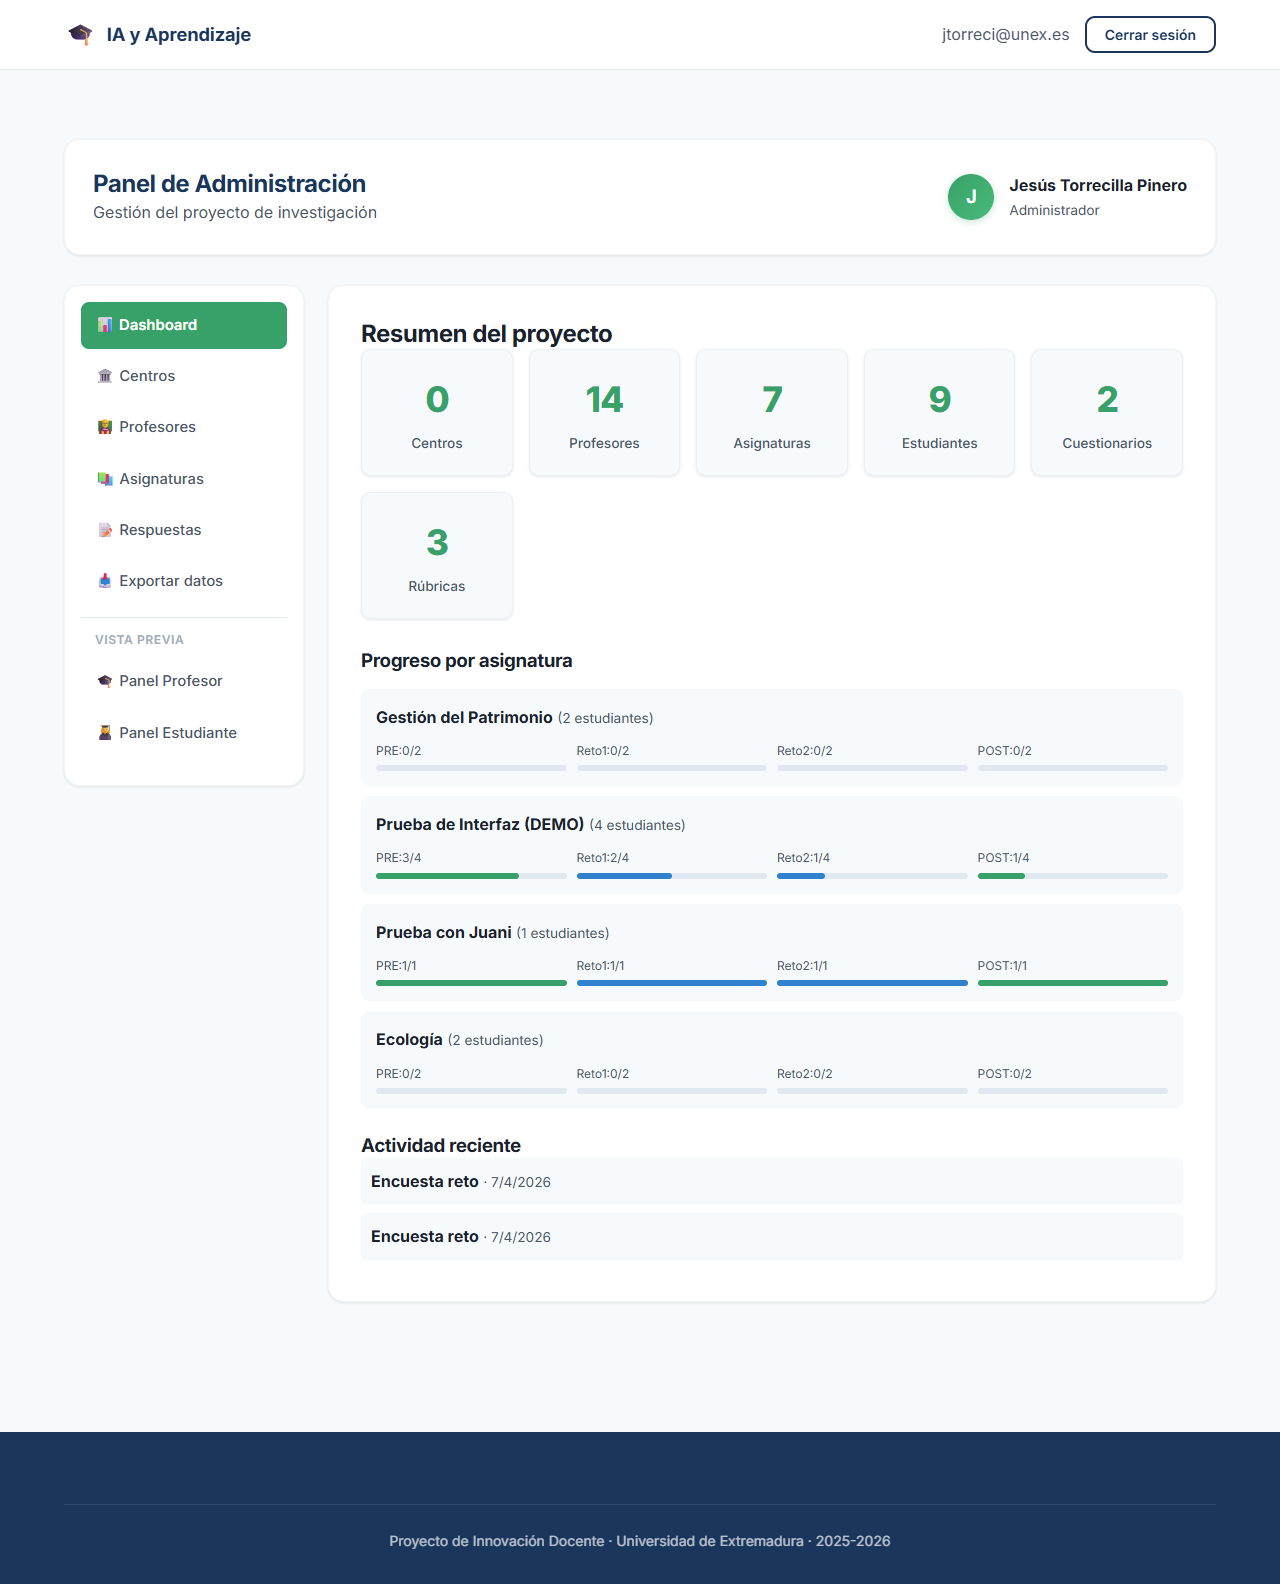
\includegraphics[width=0.85\textwidth]{05_admin_dashboard.png}}
    \caption{Panel de administración con estadísticas del proyecto y progreso por asignatura.}
\end{figure}

\seccion{Contacto y soporte}

Si tienes problemas técnicos o dudas sobre la plataforma, contacta con el equipo del proyecto:

\begin{itemize}
    \item \textbf{Web del proyecto:} \url{https://gestor-investigacion-app.web.app/participar.html}
    \item \textbf{Coordinador:} A través de la página de contacto del proyecto
\end{itemize}

\label{sec:registro}

\end{document}
